\chapterbegin{Introducción al ensamblador}
\label{chp:IntrEnsam}
\minitoc

\begin{objetivo}
En esta sesión vamos a conocer el entorno de trabajo. Veremos qué aspecto tiene un programa en ensamblador, veremos cómo funcionan los tres programas que vamos a utilizar: el ensamblador, el enlazador (linker) y el depurador (debugger). Del debugger sólo mostraremos unos pocos comandos, que ampliaremos en las próximas sesiones. También veremos la representación de los números naturales y de los enteros, y el funcionamiento de algunas de las instrucciones del ARM. Se repasarán también los conceptos de registros, flags e instrucciones para la manipulación de bits.
\end{objetivo}

\section{Lectura previa}
\label{sec:LectPrev}

\subsection{Características generales de la arquitectura ARM}
\label{sec:CaracGen}

ARM es una arquitectura RISC (Reduced Instruction Set Computer=Ordenador con Conjunto Reducido de Instrucciones) de 32 bits, salvo la versión del core ARMv8-A que es mixta 32/64 bits (bus de 32 bits con registros de 64 bits). Se trata de una arquitectura licenciable, quiere decir que la empresa desarrolladora ARM Holdings diseña la arquitectura, pero son otras compañías las que fabrican y venden los chips, llevándose ARM Holdings un pequeño porcentaje por la licencia.

El chip en concreto que lleva la Raspberry Pi es el BCM2835, se trata de un SoC (System on a Chip=Sistema en un sólo chip) que contiene además de la CPU otros elementos como un núcleo GPU (hardware acelerado OpenGL ES/OpenVG/Open EGL/OpenMAX y decodificación H.264 por hardware) y un núcleo DSP (Digital signal processing=Procesamiento digital de señales) que es un procesador más pequeño y simple que el principal, pero especializado en el procesado y representación de señales analógicas.

La CPU en cuestión es la ARM1176JZF-S, un chip de la familia ARM11 que usa la arquitectura ARMv6k. 

\begin{longtable}{| p{4.2cm} | p{2.5cm} | p{1cm} | p{6cm} |}
\hline
{\bf Familia} & {\bf Arquitectura} & {\bf Bits} & {\bf Ejemplos de dispositivos} \\ \hline
ARM1      & ARMv1       & 32/26 & Segundo procesador BBC Micro \\ \hline
ARM2, ARM3, Amber & ARMv2      & 32/26 & Acorn Archimedes \\ \hline
ARM6, ARM7 & ARMv3      & 32 & Apple Newton Serie 100 \\ \hline
ARM8, StrongARM & ARMv4       & 32 & Apple Newton serie 2x00 \\ \hline
ARM7TDMI,\newline ARM9TDMI & ARMv4T & 32 & Game Boy Advance \\ \hline
ARM7EJ, ARM9E,\newline ARM10E, XScale & ARMv5 & 32 & Samsung Omnia,\newline Blackberry 8700 \\ \hline
ARM11     & ARMv6 & 32 & iPhone 3G, Raspberry Pi \\ \hline
Cortex-M0/M0+/M1 & ARMv6-M & 32 & \\ \hline
Cortex-M3/M4 & ARMv7-M ARMv7E-M & 32 & Texas Instruments Stellaris \\ \hline
Cortex-R4/R5/R7 & ARMv7-R & 32 & Texas Instruments TMS570 \\ \hline
Cortex-A5/A7/A8/A9\newline A12/15/17, Apple A6 & ARMv7-A & 32 & Apple iPad \\ \hline
Cortex-A53/A57, X-Gene, Apple A7 & ARMv8-A & 64/32 & Apple iPhone 5S\\ \hline
\caption{Lista de familias y arquitecturas ARM}
\label{list_fam}
\endfoot
\end{longtable}

\begin{figure}[h]
  \centering
    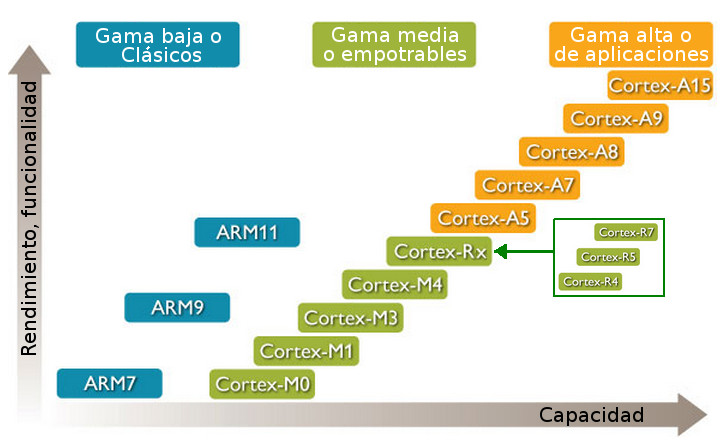
\includegraphics[width=14cm]{graphs/ArmRoadMap.jpg}
  \caption{Clasificación de Familias ARM}
  \label{fig:clasif_fami}
\end{figure}

%http://www.emcu.it/CortexFamily/ArmRoadMap.png

Las extensiones de la arquitectura ARMv6k frente a la básica ARMv6 son mínimas
\footnote{\url{http://infocenter.arm.com/help/index.jsp?topic=/com.arm.doc.ddi0301h/apbs02s02.html}}
por lo que a efectos prácticos trabajaremos con la arquitectura ARMv6.

\subsection{Registros}
\label{sec:Registros}

La arquitectura ARMv6 presenta un conjunto de 17 registros (16 principales más uno de estado) de 32 bits cada uno. A nivel interno son 40 registros, pero los restantes 23, también llamados registros encauzados o banked registers, se basan en copias de los 17 principales. Como nosotros vamos a programar dentro de un sistema operativo, emplearemos básicamente el modo usuario, por lo que no entraremos en detalle de los otros modos de operación que tiene la CPU, y por tanto trabajaremos sólo con los 17 registros indicados.

\begin{figure}[h]
  \centering
    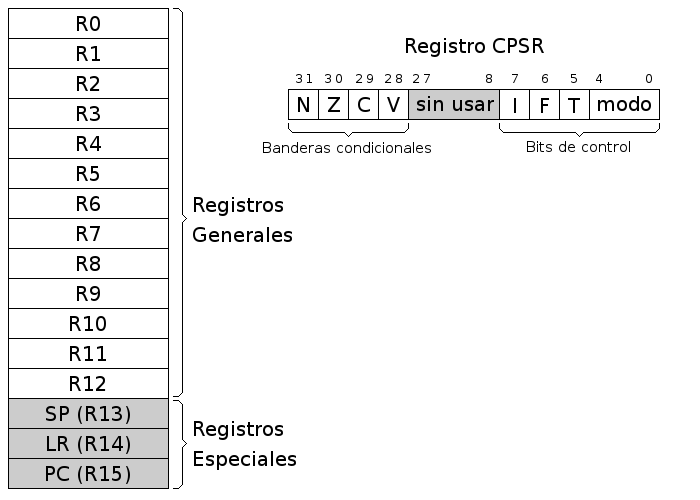
\includegraphics[width=8cm]{graphs/registros.png}
  \caption{Registros de la arquitectura ARM}
  \label{fig:reg_arm}
\end{figure}


\chapterend{}
